\documentclass{beamer}
\DeclareFontShape{OT1}{cmss}{b}{n}{<->ssub * cmss/bx/n}{} 
\usetheme{default}
\usepackage{amsmath}
\usepackage{amsfonts}
\usepackage{mathbbol}
\usepackage{xcolor} % before tikz or tkz-euclide if necessary
\usepackage{tkz-euclide} % no need to load TikZ
\usepackage{multirow}
\usepackage{bm}


\usepackage[
backend=biber,
style=authoryear-icomp,
sortlocale=de_DE,
natbib=true,
url=false, 
doi=true,
eprint=false
]{biblatex}
\addbibresource{../../Bibliography/main_ML.bib}

\titlegraphic{\includegraphics[width=2cm]{../../Figures/UAMS_RGB.png}
}

\title{Statistical Machine Learning\\ Manifold Learning}
\author{Horacio G\'omez-Acevedo\\ Department of Biomedical Informatics}
\begin{document}
	\begin{frame}[plain]
		\maketitle
	\end{frame}
\begin{frame}{Linear Models}
	Popular methods of data analysis make the assumption that the data lies on a linear $k$-dimensional subspace of $\mathbb{R}^n$ where $k< n$. 
	
	The general problem reduces to search for a linear transformation $\theta \colon \mathbb{R}^n \to \mathbb{R}^k$ such that $\{\theta(x_i)\}$ retains something about the structure of $\{x_i\}$. 
	
	Linear models are ubiquitous in sciences, but the assumption of linearity is often unrealistic. One alternative, is to consider that the data has been sampled from a (compact Riemannian) \textbf{manifold} ${\cal M}\subset \mathbb{R}^n$ of much lower dimension than $n$. 

\end{frame}

\begin{frame}{What is a manifold?}
	Roughly speaking, a manifold (of dimension 2) is a surface that locally behaves as a regular space in $\mathbb{R}^2$. In geometry, we refer to local properties as intrinsic. 
\begin{figure}[h]
	\centering
	\includegraphics[width=7cm]{../../Figures/fig_manifold.jpg}
\end{figure}	
		
\end{frame}

\begin{frame}{The Sphere as a manifold}
	Another typical example is the sphere (often called $S^2$).
	
\begin{figure}[h]
	\centering
	\includegraphics[width=7cm]{../../Figures/fig_manifold_sphere.jpg}
\end{figure}	
Intuitively, we cannot cover the whole sphere (in a unique way) with only one sheet. The north and south poles are a problem. 

\end{frame}

\begin{frame}{Sphere as a patch work}
	Instead, we use several overlapping sheets 
\begin{figure}[h]
	\centering
	\includegraphics[width=6cm]{../../Figures/fig_manifold_sphere_2.jpg}
\end{figure}		
	
	
\end{frame}

\begin{frame}{Manifold Learning }
	
	Loosely speaking, the basic idea of most manifold learning techniques is to take the $k$-nearest neighbors of a point $x$ and use the vectors specified by the line segments from $x$ to its neighbors as an approximation for the tangent plane at $x$. 
	
	Global optimization then sews these local approximations together to produce a low-dimensional representation of the data. 
	
\begin{center}
\textbf{Manifold learning is also known as dimensionality reduction.} 
\end{center}
\end{frame}


\begin{frame}{PCA}
	In a general setup, we can think that we have $m$ vectors in $\mathbb{R}^n$, namely $\{x_1, \ldots, x_m\}$. We try to find the "optimal" linear projection $\theta \colon \mathbb{R}^n \to \mathbb{R}^k$ where $k \ll n$ (meaning $k$ much lower than $n$)
	\begin{enumerate}
	\item $\tilde{x_j} = x_j -\mu$ where $\mu= \frac{1}{m} \sum x_j$
	\item We find the variance-covariance matrix 
	\begin{equation*}
		C=\frac{1}{m} \sum_{j=1}^m \tilde{x_j} \tilde{x_j}^t
	\end{equation*}
	\item We compute the top $k$-eigenvectors $\{v_1, \ldots, v_k\}$ of $C$.
	\item These eigenvectors span a hyperplane (subspace) of $\mathbb{R}^n$. The projection $\theta \colon \mathbb{R}^n \to \mathbb{R}^k$ is precisely the orthogonal projection onto this plane followed by a choice of identification of the plane with $\mathbb{R}^k$.
	\item We can think $\theta$ as 
	\begin{equation*}
		y_j= \theta(\tilde{x_j})+ \mu
	\end{equation*}
	
	\end{enumerate}


\end{frame}

\begin{frame}{PCA cont}
	The process chooses the basis which maximizes the variance captured by the representation; the eigenvector $v_1$ with the largest eigenvalue is the single direction that captures the maximal amount of information about the variance; the plane spanned by $\{v_1,v_2\}$ is the plane with the most variance, etc.
	
	Another characterization of PCA is to find a projection that minimizes the error function
	\begin{equation*}
		E= \sum_{j=1}^m \| x_j -y_j \|^2, 
	\end{equation*}
	where $\| \cdot \|$ denotes some distance. For PCA this means that it produces the points $\{y_i\}$ that minimize the reconstruction error among all projections onto a $k$ dimensional subspace. 
\end{frame}

\begin{frame}{Multidimensional scaling (MDS)}
	
From Lapedes and Farber (2001)
\begin{quote}
	``Multidimensional scaling'' algorithms are a class of algorithms
	initially developed in the computational psychology literature (Shepherd, 1963, 1964) which reconstruct the true dimension of the space, and the
	relative coordinates of points, given only distances, or more generally monotonic transformations of distances, between the points. ``Relative''
	means that coordinates are reconstructed from
	the distance data up to global translation, reflection, scale and rotation which leave the relative
	relation of points invariant. Since interest centers
	on relative relationships, such global transformations are irrelevant.
\end{quote}
	
\end{frame}

\begin{frame}{MDS formally}

In this methodology, we search for a mapping $\theta \colon \mathbb{R}^n \to \mathbb{R}^k$ that minimizes
\begin{equation*}
	{\cal E}= \sum_{x_i,x_j} ( d(x_i,x_j) - \|\theta(x_i)-\theta(x_j)\|)^2,
\end{equation*}
where $d$ is an (intrinsic) distance. 
The procedure is as follows. 
\begin{enumerate}
	\item Consider the matrix of the original distances $D=(D_{ij})$ where $D_{ij}= d(x_i,x_j)$. 
	\item Set $H= I_n - \frac{1}{n} \mathbb{1} \cdot \mathbb{1}^t$, where $\mathbb{1}= (1,1, \ldots, 1)$. Set $Z= -\frac{1}{2} H D H$.
	\item The function that minimizes $\cal E$ is then given by finding the eigenvectors $v_j$ of $Z$. The $\theta(x_j)$ is specified by normalizing so that $\|v_j\|^2=\lambda_j$.
\end{enumerate}
\end{frame}

\begin{frame}{MDS (cont)}

\begin{figure}[h]
	\centering
	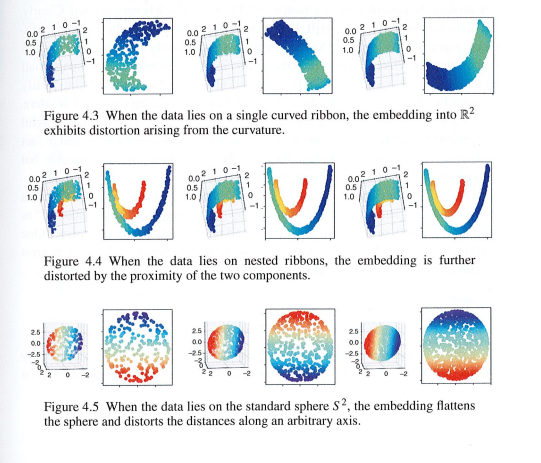
\includegraphics[width=7cm]{../../Figures/fig_mds_manifold.png}
\end{figure}

\begin{theorem}
	Given $\{x_1, \ldots, x_l\}\subset \mathbb{R}^n$ and $k<$, the results of metric MDS and PCA embedding $\{x_i\}$ into $\mathbb{R}^k$ are isometric.
\end{theorem}

\end{frame}
\begin{frame}{Manifold Learning Main Ideas}
	Suppose that we are given data points $\{x_1, \ldots, x_m\}$ in $\mathbb{R}^n$. We will assume that there is a function (embedding) $\gamma \colon {\cal M} \to \mathbb{R}^n$. 
	
	Keep in mind that \textit{distances} in manifolds can be different
\begin{figure}[h]
	\centering
	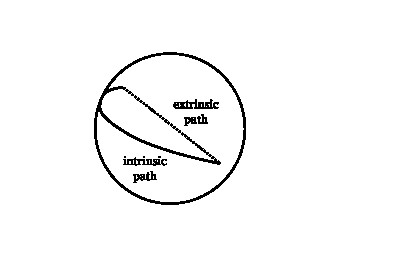
\includegraphics[width=3cm]{../../Figures/fig_geodesic.jpg}
\end{figure}
	The manifold structure can be reconstructed by considering the "short distances" as reliable indicators of the local (intrinsic) distances and ignoring the "long distances".
	

\end{frame}


\begin{frame}{Isomap}
	Isomap applies MDS to an empirical approximation of the intrinsic metric.
	The procedure goes as follows. We fix a scale parameter $\varepsilon$ and a target dimension parameter $k$.
	
	\begin{enumerate}
		\item Form the weighted graph $G$ with
		\begin{itemize}
			\item vertices the points $\{x_i\}$, and
			\item edges $(i,j)$ with weights given by $w_{ij}=\| x_i -x_j\|$ when $\|x_i -x_j\| \le \varepsilon$.
		\end{itemize}
		\item We form a new space $X'$ with points $\{x_i\}$ but distances given by the graph metric on $G$.  Meaning that the distances between two edges is given by the shortest path in the graph.
		\item Use MDS to embed this space into $\mathbb{R}^k$ producing points $y_i = \theta(x_i)$
	\end{enumerate}
\end{frame}

\begin{frame}{Isomap}
	\begin{figure}[h]
		\centering
		\includegraphics[width=10cm]{../../Figures/fig_manifolde_4_7.jpg}
	\end{figure}	
\end{frame}

\begin{frame}{Isomap cont.}
		\begin{figure}[h]
		\centering
		\includegraphics[width=10cm]{../../Figures/fig_manifolde_4_8.jpg}
	\end{figure}	
\end{frame}

\begin{frame}{Local Linear Embedding LLE}
	We fix a target dimension parameter $k$ and a neighborhood size $K$. The algorithm goes as follows:
	\begin{enumerate}
		\item For each point $x_i$, we solve for weight $w_{ij}$ which minimize the expression
		\begin{equation*}
			{\cal E}(x_i)= \sum_i \left( x_i - \sum_j w_{ij} x_j \right)^2, 
		\end{equation*}
		subject to the constrains
		\begin{equation*}
			\begin{cases}
				w_{ij}=0 & \text{$x_j$ not a $K$ nearest neighbor of $x_i$}.\\
				\sum_j w_{ij}=1 & \\
			\end{cases}
		\end{equation*}
	We are solving for weights that optimally reconstruct each point $x_i$ from its $K$ nearest neighbors. The weights can efficiently computed via least squares.
	\item Embedding points $\{ y_i = \theta(x_i)\} \subset \mathbb{R}^k$ are computed so that

	\end{enumerate}
\end{frame}

\begin{frame}{LLE cont.}
		\begin{equation*}
		{\cal E}= \sum_i \left( y_i - \sum_j w_{ij}y_j \right)^2
	\end{equation*}

		is minimized. To solve this problem we can calculate the top $k$ eigenvectors of the corresponding matrix of the quadratic form. 
	\begin{figure}[h]
	\centering
	\includegraphics[width=8cm]{../../Figures/fig_manifolde_4_10.jpg}
\end{figure}			
		
\end{frame}

\begin{frame}{LEE cont}
		\begin{figure}[h]
		\centering
		\includegraphics[width=8cm]{../../Figures/fig_manifolde_4_11.jpg}
	\end{figure}			
\end{frame}


\begin{frame}{Neighbor Embedding Algorithms}
	These algorithms aim to address the problem when data points have non-uniform density. The \textbf{stochastic neighbor embedding (SNE)} and the \textbf{$t$-distributed stochastic neighbor embedding (t-SNE)} aim to address that issue.
	
	We begin with our traditional setup for data where $\{x_i\} \subset \mathbb{R}^n$ and $\{y_i\} \subset \mathbb{R}^k$, where $k \le n$ (hopefully considerably smaller). Then we define
	\begin{equation*}
		p_{j|i}= \frac{ \exp( \frac{- \|x_i -x_j\|^2}{2\sigma_i^2})}{ \sum_{k\ne i}\exp( \frac{- \|x_i -x_j\|^2}{2\sigma_i^2})}
	\end{equation*}
	and
	\begin{equation*}
		q_{j|i}= \frac{ \exp( - \|y_i -y_j\|^2)}{ \sum_{k\ne i}\exp( - \|y_i -y_j\|^2)}
	\end{equation*}
		where the variances $\sigma_i$ are obtained by an optimization process, and in the second equation we are fixing all of the variances to be identically $\sqrt{2}/2$. 
\end{frame}
\begin{frame}{SNE cont.}
	The idea behind SNE is that good image points $\{y_i\}$ have the property that the difference between $p_{j|i}$ and $q_{j|i}$ is minimized in the sense of the so-called summed Kullback-Leibler divergences cost function
	\begin{equation*}
		C= \sum_i \sum_j p_{j|i} \log \frac{p_{j|i}}{q_{j|i}}
	\end{equation*} 
	This equation ensures that the local distributions have similar means. 
	
	

\end{frame}

\begin{frame}{SNE cont}
	
	In practice, SNE algorithm proceeds by solving the minimizing point $\{y_i\}$ via a gradient descent in order to find a good local minimum for $C$.  Convergence is often slow and depends critically on good choices of the variances $\sigma_i$. In principle, differing choices of $\sigma_i$amount to enforcing variable numbers of neighbors used to do the local estimation of the coordinates; this is expressed here via the use of the \textbf{perplexity} which is computed as
	\begin{equation*}
		P= 2^{- \sum_j p_{j|i}\log_2 p_{j|i}}
	\end{equation*}
	The desired perplexity is typically between 10 and 100 is a parameter and we solve for values $\sigma_i$ that achieve the perplexity.

\end{frame}

\begin{frame}{$t$-SNE}
	One problem with the original SNE is that the gradient descent optimization is slow and difficult to achieve convergence. The proposed solution goes as follows
	\begin{enumerate}
		\item We symmetrize $p_{j|i}$ as 
		\begin{equation*}
			p_{ij}= \frac{p_{j|i}+p_{i|j}}{2}
		\end{equation*}
	\item We define a symmetrize variant of $q_{j|i}$ as follows
	\begin{equation*}
		q_{ij}= \frac{(1+\|y_i-y_j\|^2)^{-1}}{\sum_{k\ne l}(1+\|y_k-y_l\|^2)^{-1}}
	\end{equation*}
	In the original definition, the $q_{j|i}$ was defined using a Gaussian; this expression replaces that with the Student $t$-distribution with one degree of freedom, which has more weight in the tails.
	\item Finally, the cost function is replaces with the expression
	\begin{equation*}
		C= \sum_i \sum_j p_{ij} \log \frac{p_{ij}}{q_{ij}}
	\end{equation*}
	\end{enumerate}
\end{frame}

\begin{frame}{$t$-SNE advantages over SNE}
	Why do we complicate things this way?
	\begin{enumerate}
		\item The use of a heavier tailed distribution means that outliers have less impact on the overall results and the compression effects around the center of mass are alleviated (to some degree)
		\item The adjusted formula for $q_{ij}$ also has the effect of substantially improving the efficiency and quality of the gradient descend procedure.
	\end{enumerate}
\end{frame}

\begin{frame}{$t$-SNE cont}
	\begin{figure}[h]
		\centering
		\includegraphics[width=8cm]{../../Figures/fig_manifolde_4_17.jpg}
	\end{figure}				
	
\end{frame}


\begin{frame}{What we have learned?	}
	\begin{itemize}
		\item Manifold learning and dimensionality reduction are similar concepts.
		\item The idea is to reduce dimensionality taking advantage of the manifold structure of our data. 
		\item Most of these methods imply that we can understand the local behavior of our data and classical methodologies are applied based on this assumption.
	\end{itemize}
\end{frame}



\begin{frame}{References}
	Some of the pictures are from \citep{docarmoriemann}, and \citep{schutz}, and \citep{geron2}. Main reference for manifold learning \citep{rabadan}.
	\printbibliography 	
	
	I have used some of the graphs by hacking TiKz code from StakExchange, Inkscape for more aesthetic plots and other old tricks of \TeX
	
\end{frame}


	
\end{document}
